\section{Benutzerschnittstelle}

\subsection{Einführung}
Die Benutzeroberfläche muss so aufgebaut sein, dass auch unerfahrene Benutzer das System problemlos verwenden können.
Um die Benutzerführung zu optimieren werden insbesondere sog. "Wizards" verwendet. In diesen wird der Benutzer dann durch die verschiedenen Schritte eines gegebenen Ablaufs geführt. Darüber hinaus wird an vielen Stellen das Drag-and-Drop-Konzept verwendet.
Hierdurch wird die Benutzeroberfläche intuitiver und die Dauer der einzelnen Interaktionen des Nutzers mit dem System wird verkürzt.
\subparagraph{}
Alle Angaben zur Benutzeroberfläche sind vorläufig, da auch viele der Wunschkriterien aus Kapitel \ref{subsec:project_goals-wunschkriterien} in dieser Oberfläche realisiert werden. Die exakte visuelle Ausgestaltung der Elemente ist ebenfalls vorläufig.
\subsection{Login}
\begin{figure}[!htb]
	\caption{Loginseite des Systems mit Anmeldung über den Shibboleth Identity Provider des KITs}
	\label{fig:gui-login-1}
	\centering
	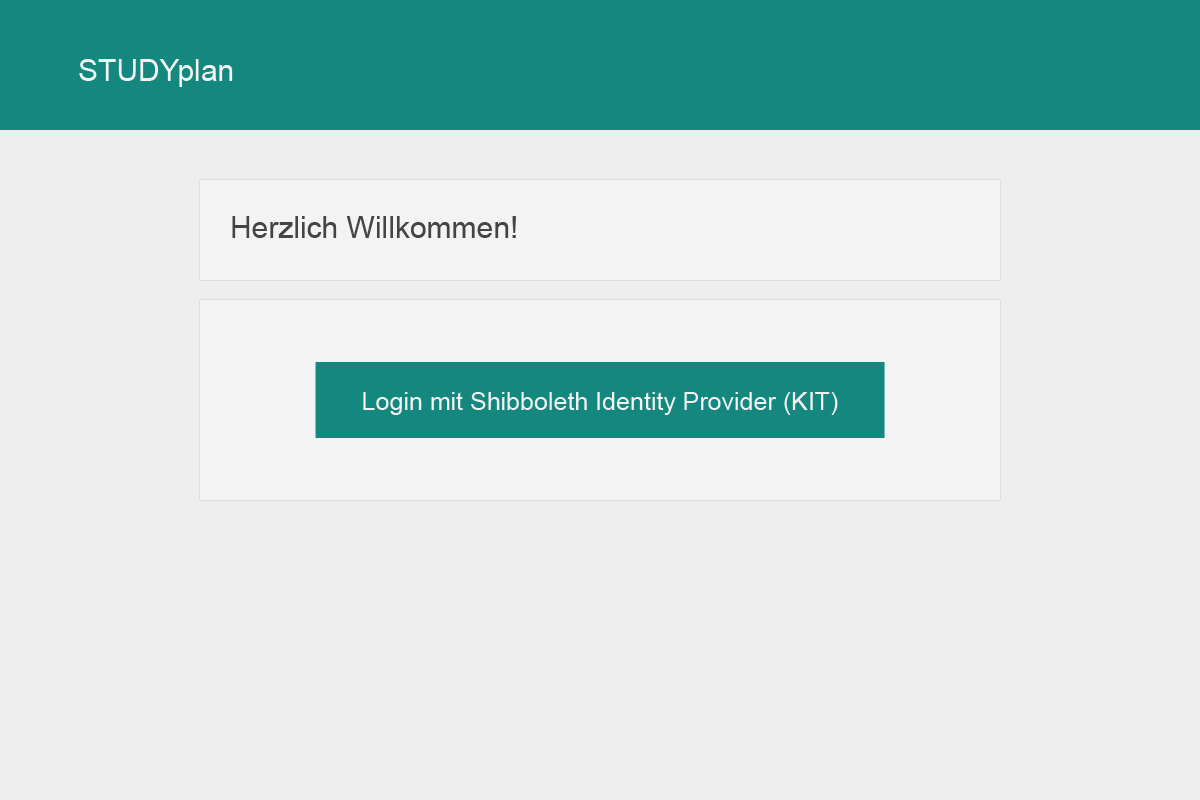
\includegraphics[width=0.7\textwidth]{../GUI/ergebnisse/login-1.png}
\end{figure}
Abbildung \ref{fig:gui-login-1} zeigt die Login-Seite. Diese sollte recht minimalistisch sein und lediglich die Möglichkeit bieten sich mit Hilfe des Shibboleth-Identity-Providers des KITs einloggen zu können.
\subparagraph{}
Loggt sich der Nutzer zum ersten Mal in das System ein wird er zum Registrierungs-Wizard (siehe Kapitel \ref{subsec:gui-registrierung}) weitergeleitet. Wenn er sich bereits zuvor schon einmal eingeloggt hat wird er auf die Hauptseite (siehe Kapitel \ref{subsec:gui-hauptseite}) weitergeleitet.
\subsection{Registrierungs-Wizard}
\label{subsec:gui-registrierung}
Nach dem Login wird man zum Registrierungs-Wizard weitergeleitet. Auf der ersten Seite (Abbildung \ref{fig:gui-registrierung-1}) wird der Nutzer dort nach grundlegenden Informationen wie dem Studiengang und dem Semester des Studienbeginns gefragt. Die Eingabe dieser Daten ist verpflichtend.
\subparagraph{}
Nachdem der Nutzer dann auf den Pfeil in der unteren Ecke geklickt hat, wird er auf die zweite Seite des Wizards (Abbildung \ref{fig:gui-registrierung-2}) weitergeleitet. Hier kann er angeben, welche Module er bereits begonnen und/oder abgeschlossen hat. 
Nach dem Bearbeiten der zweiten Seite des Wizards und dem Klick auf den Pfeil, wird der Nutzer auf die Hauptseite des Systems (siehe Kapitel \ref{subsec:gui-hauptseite}) weitergeleitet.
\subparagraph{}
Durch den Wizard soll sichergestellt werden, dass der Nutzer alle für das System relevanten Daten eingibt bevor er mit der Nutzung beginnt.
\begin{figure}[!htb]
	\caption{Erste Seite des Registrierungs-Wizard mit Eingabe von Studienfach und Studienbeginn}
	\label{fig:gui-registrierung-1}
	\centering
	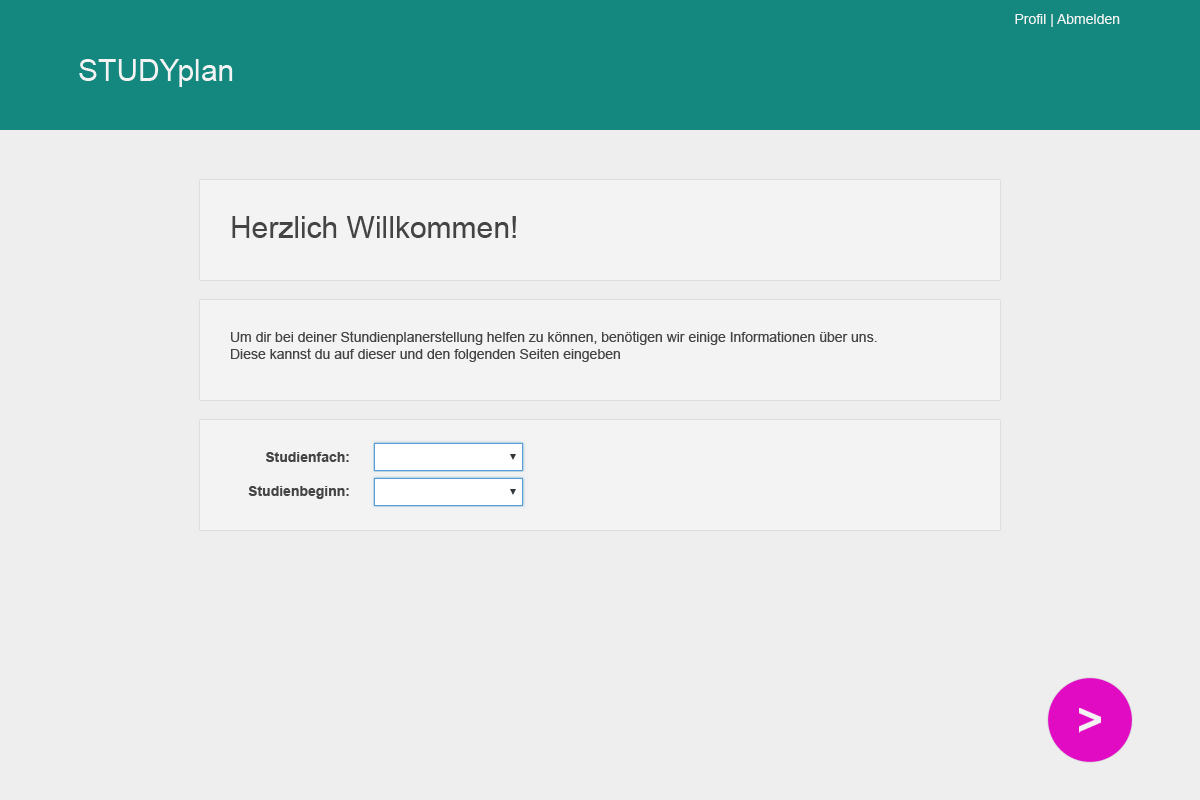
\includegraphics[width=0.7\textwidth]{../GUI/ergebnisse/registrierung-1.png}
\end{figure}

\begin{figure}[!htb]
	\caption{Zweite Seite des Registrierungs-Wizard mit Eingabe der schon begonnenen Module}
	\label{fig:gui-registrierung-2}
	\centering
	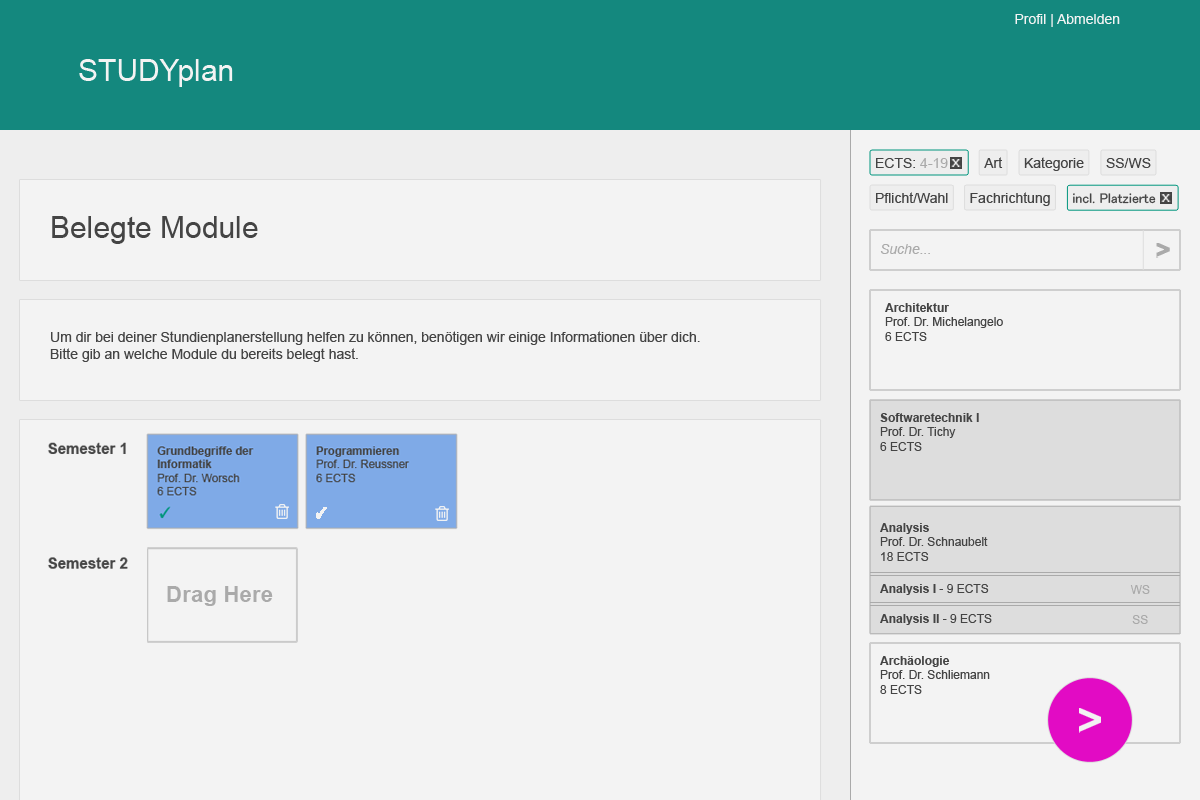
\includegraphics[width=0.7\textwidth]{../GUI/ergebnisse/registrierung-2.png}
\end{figure}


\subsection{Hauptseite}
\label{subsec:gui-hauptseite}
Die Hauptseite des Systems (Abbildung \ref{fig:gui-hauptseite-1}) stellt für den Nutzer die zentrale Anlaufstelle für alle Anwendungsfälle dar. Der Nutzer kann auf dieser Seite seine vorhandenen Studienpläne anzeigen, duplizieren, löschen sowie exportieren. Über das selektieren von mehreren Plänen, kann er auch Pläne vergleichen oder mehrere gleichzeitig löschen. Mittels des Plus-Buttons kann er darüber hinaus neue Pläne erstellen.\newline
Beim Klick auf "Anzeigen" wird der Nutzer auf die Seite zur manuellen Bearbeitung von Studienplänen (siehe Kapitel \ref{subsec:gui-manuelle-bearbeitung}) geleitet. Beim Klick auf das "+" wird er nach einem Namen für die Seite gefragt und anschließend ebenfalls auf die Seite zur manuellen Bearbeitung weitergeleitet.
\begin{figure}[!htb]
	\caption{}
	\label{fig:gui-hauptseite-1}
	\centering
	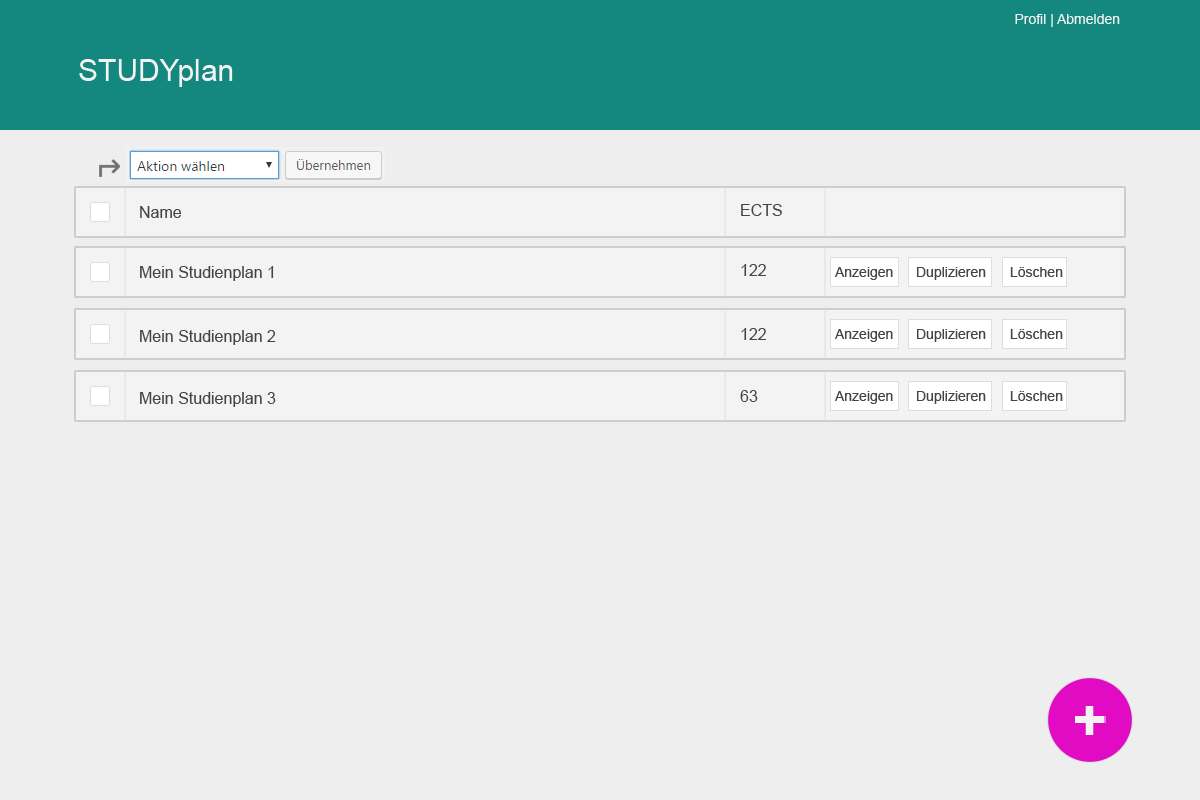
\includegraphics[width=0.7\textwidth]{../GUI/ergebnisse/hauptseite-1.png}
\end{figure}

\subsection{Manuelle Studienplan-Bearbeitung}
\label{subsec:gui-manuelle-bearbeitung}
In dieser Ansicht (Abbildung \ref{fig:gui-bearbeitung-1}) ist es dem Nutzer möglich, seinen Studienplan manuell zu bearbeiten. Hierfür kann er mittels Drag-and-Drop Module oder Teilmodule (z.B. das Teilmodul Analysis I in der Abbildung) in das gewünschte Semester zu ziehen. Hierdurch wird es dem Studienplan hinzugefügt.
\begin{figure}[!htb]
	\caption{}
	\label{fig:gui-bearbeitung-1}
	\centering
	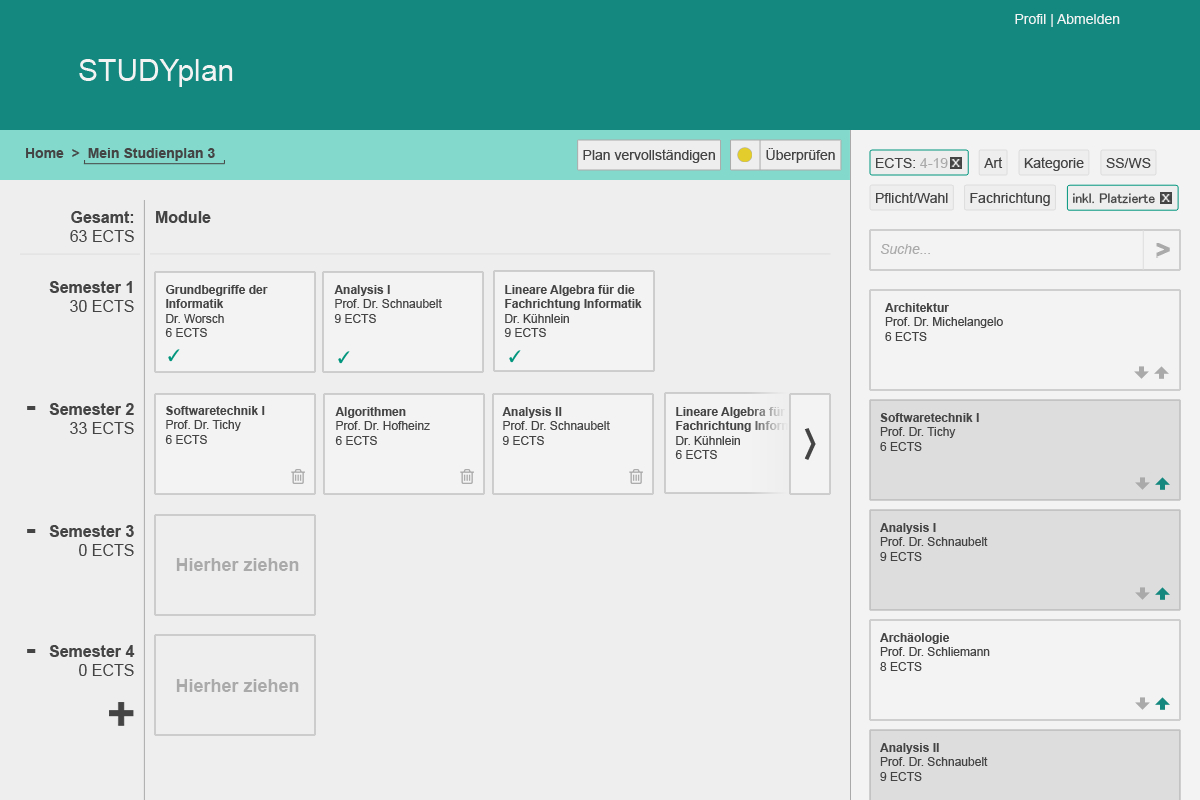
\includegraphics[width=0.7\textwidth]{../GUI/ergebnisse/bearbeitung-1.png}
\end{figure}

\subsubsection{Module filtern}
Module sind filterbar.
\begin{figure}[!htb]
	\caption{}
	\label{fig:gui-module-filtern-1}
	\centering
	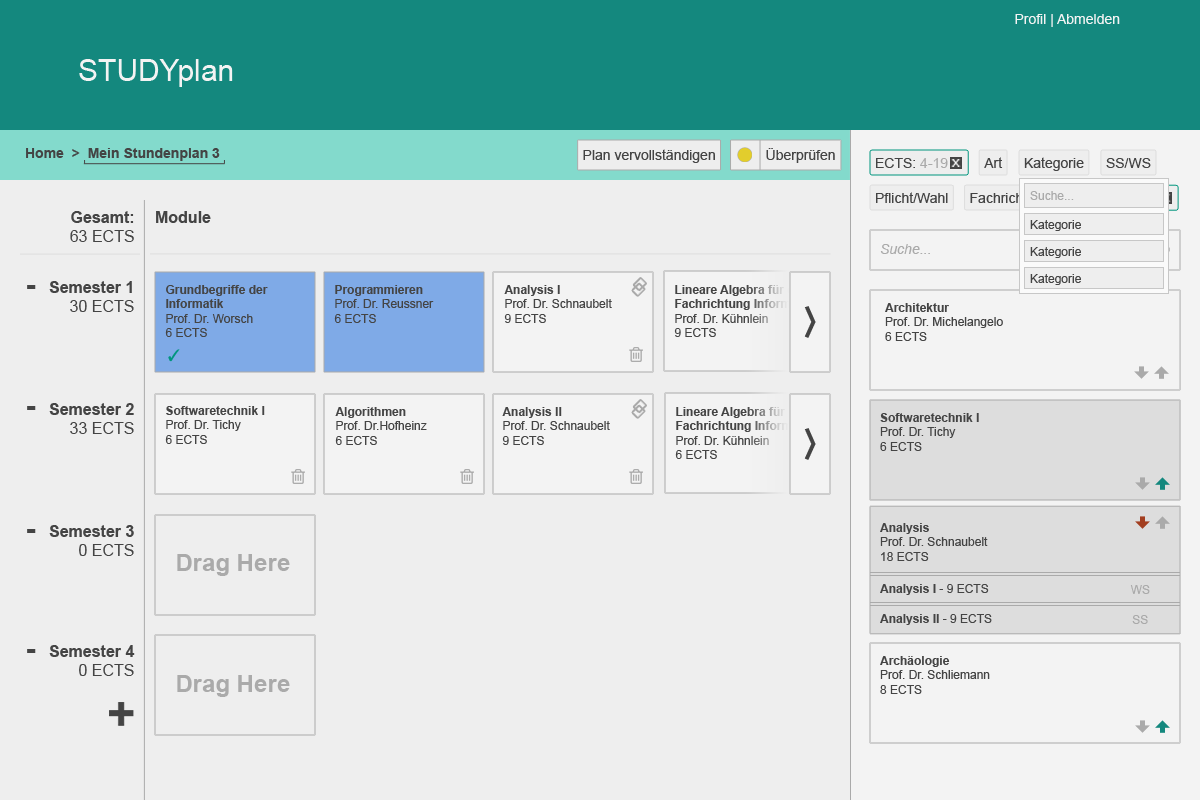
\includegraphics[width=0.7\textwidth]{../GUI/ergebnisse/module-filtern-1.png}
\end{figure}
\begin{figure}[!htb]
	\caption{}
	\label{fig:gui-module-filtern-2}
	\centering
	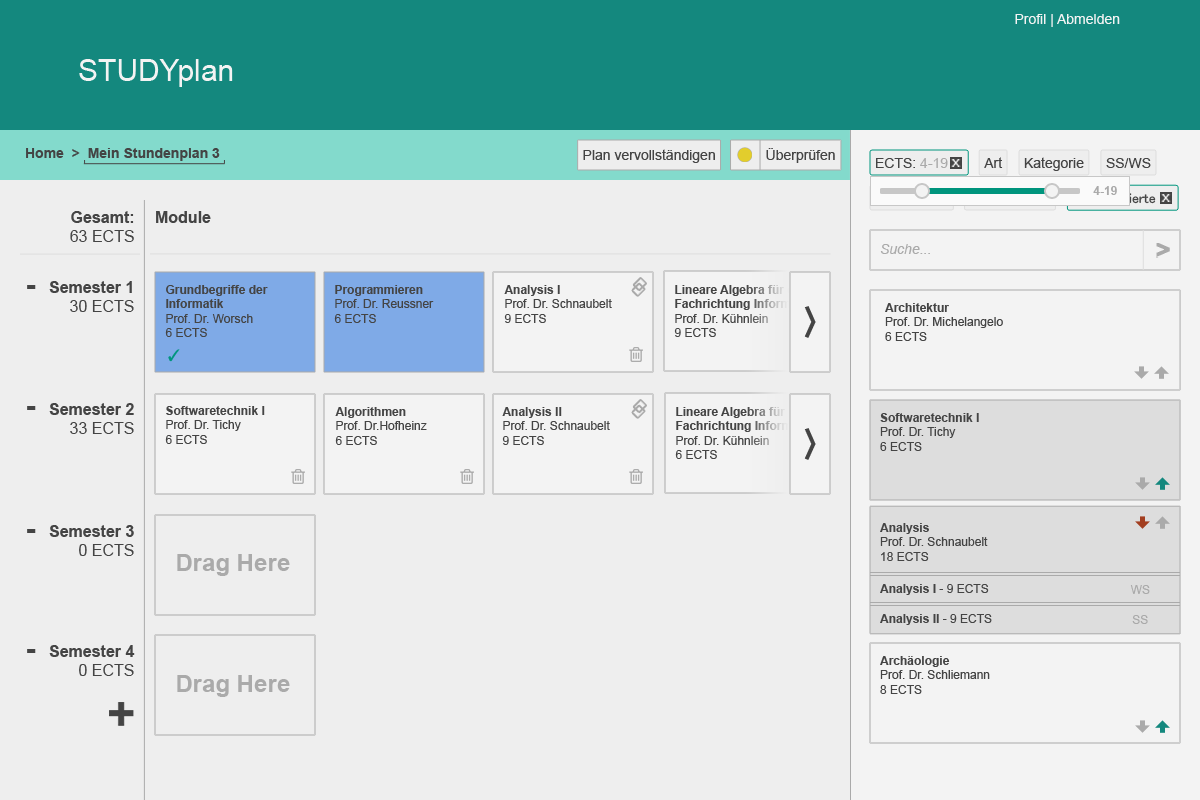
\includegraphics[width=0.7\textwidth]{../GUI/ergebnisse/module-filtern-2.png}
\end{figure}

\subsubsection{Modul-Informationen anzeigen}
Modulinformationen lassen sich auch anzeigen
\begin{figure}[!htb]
	\caption{}
	\label{fig:gui-modul-info-1}
	\centering
	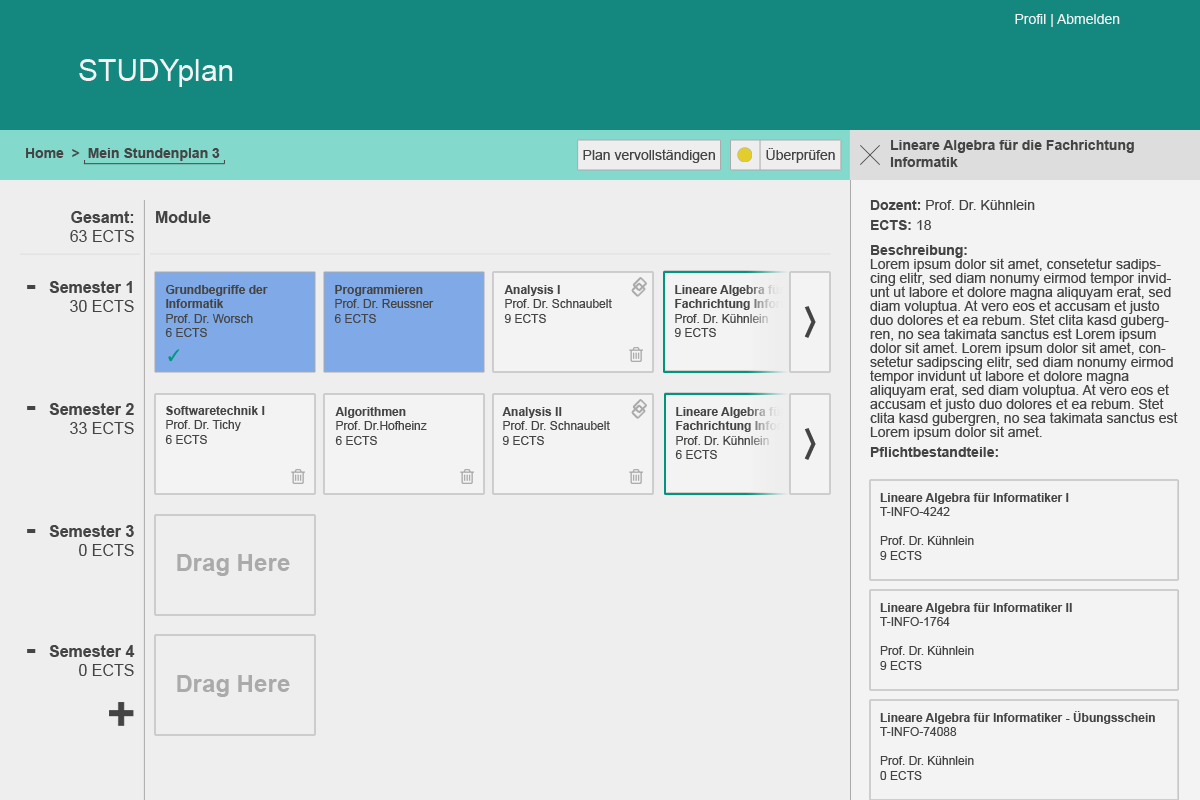
\includegraphics[width=0.7\textwidth]{../GUI/ergebnisse/modul-info-1.png}
\end{figure}


\subsection{Generierungs-Wizard}
Hier kann man Stundenpläne generieren.
\begin{figure}[!htb]
	\caption{}
	\label{fig:gui-generierung-1}
	\centering
	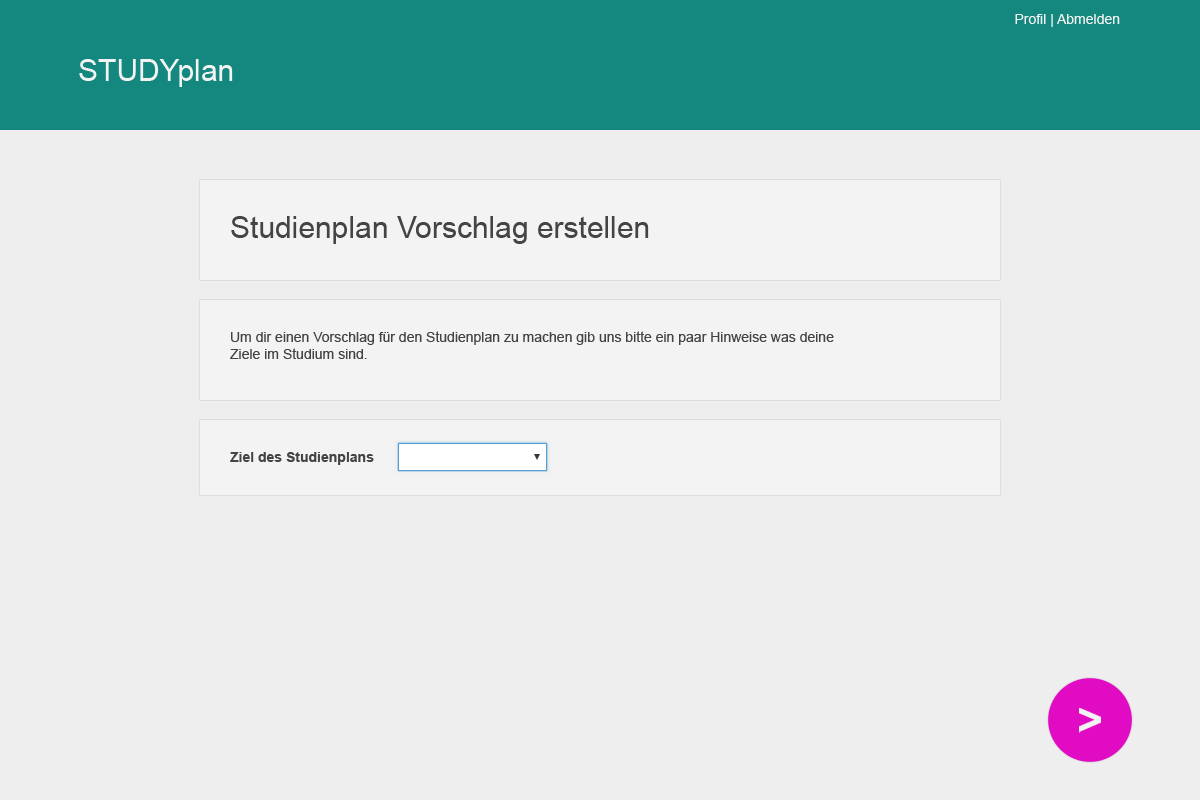
\includegraphics[width=0.7\textwidth]{../GUI/ergebnisse/generierung-1.png}
\end{figure}

\begin{figure}[!htb]
	\caption{}
	\label{fig:gui-generierung-2}
	\centering
	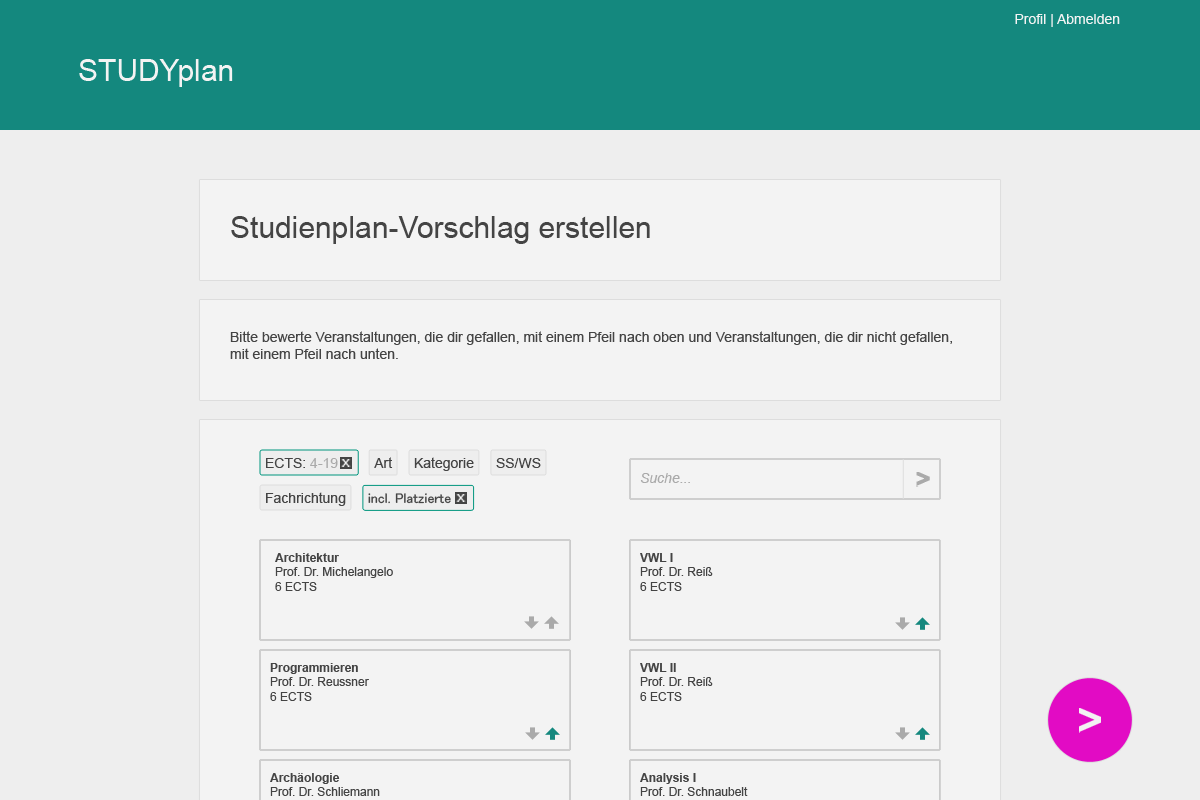
\includegraphics[width=0.7\textwidth]{../GUI/ergebnisse/generierung-2.png}
\end{figure}

\begin{figure}[!htb]
	\caption{}
	\label{fig:gui-generierung-3}
	\centering
	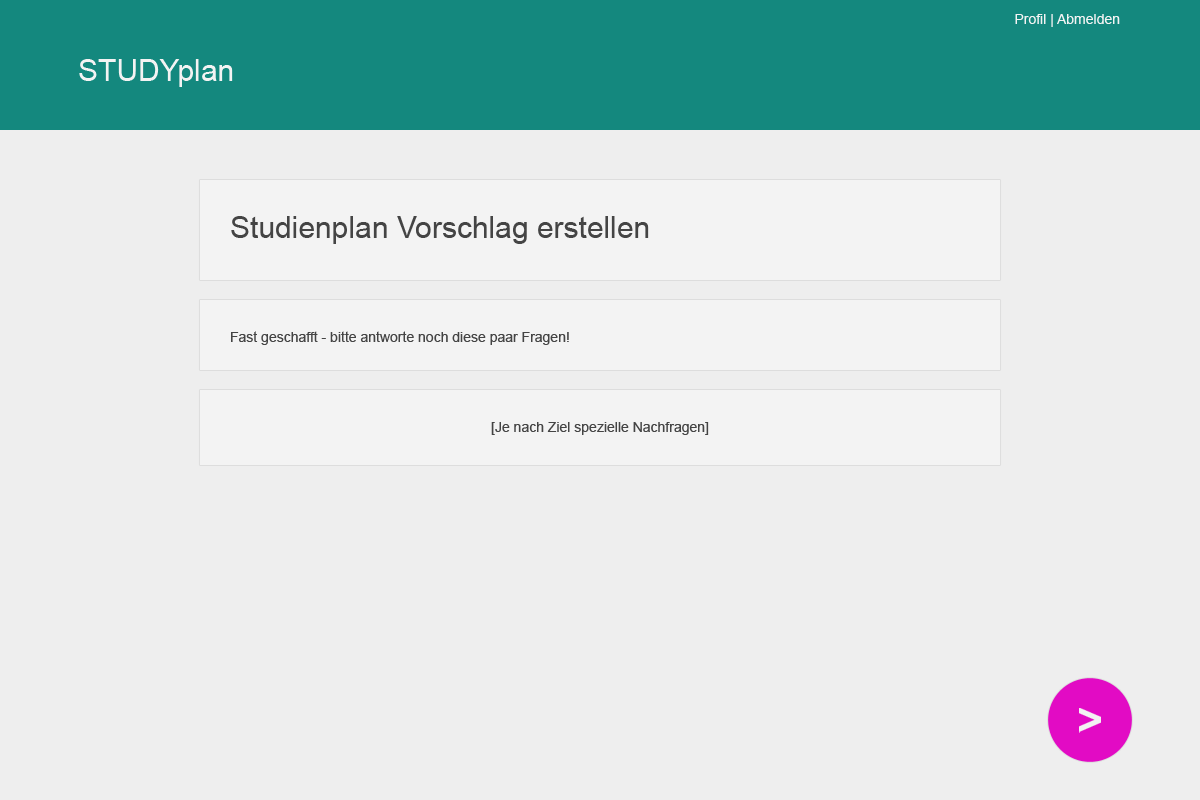
\includegraphics[width=0.7\textwidth]{../GUI/ergebnisse/generierung-3.png}
\end{figure}

\begin{figure}[!htb]
	\caption{}
	\label{fig:gui-generierung-4}
	\centering
	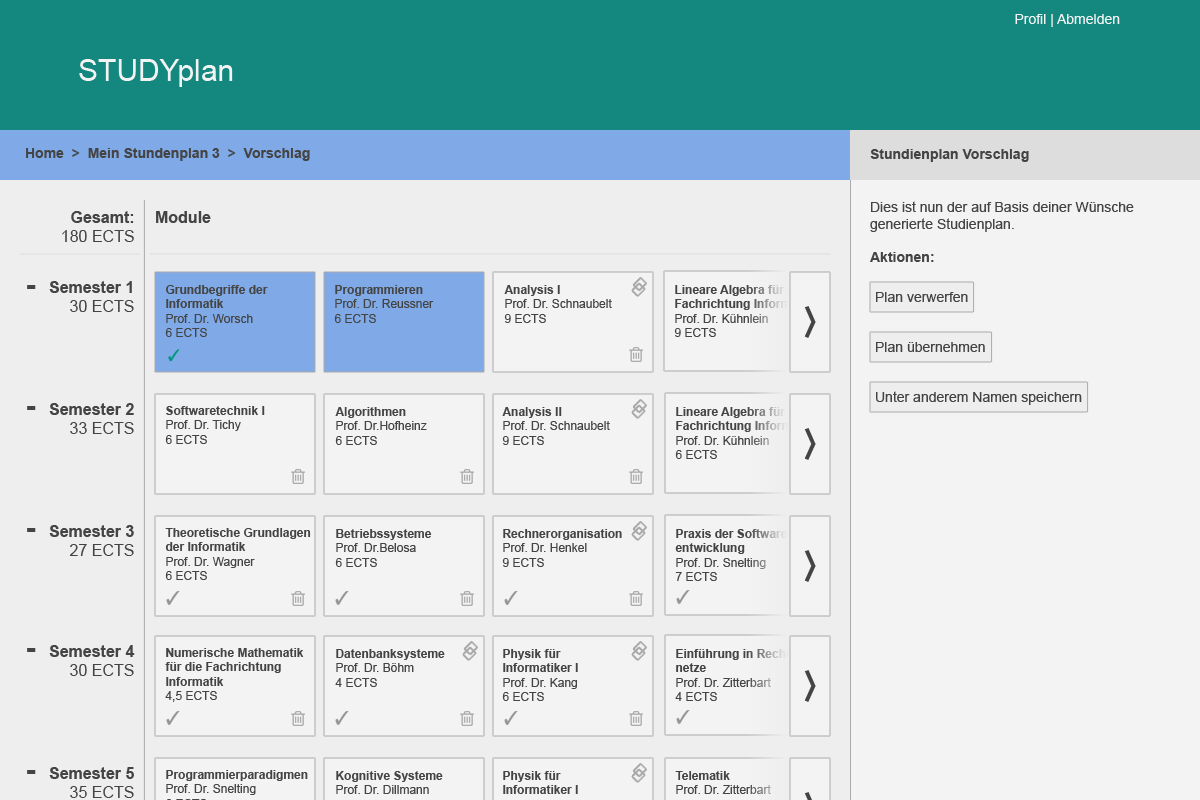
\includegraphics[width=0.7\textwidth]{../GUI/ergebnisse/generierung-4.png}
\end{figure}

\subsection{Verifizierung}
Verifizierung ist auch möglich mittels dieser Darstellung.
\begin{figure}[!htb]
	\caption{}
	\label{fig:gui-verifizierung-1}
	\centering
	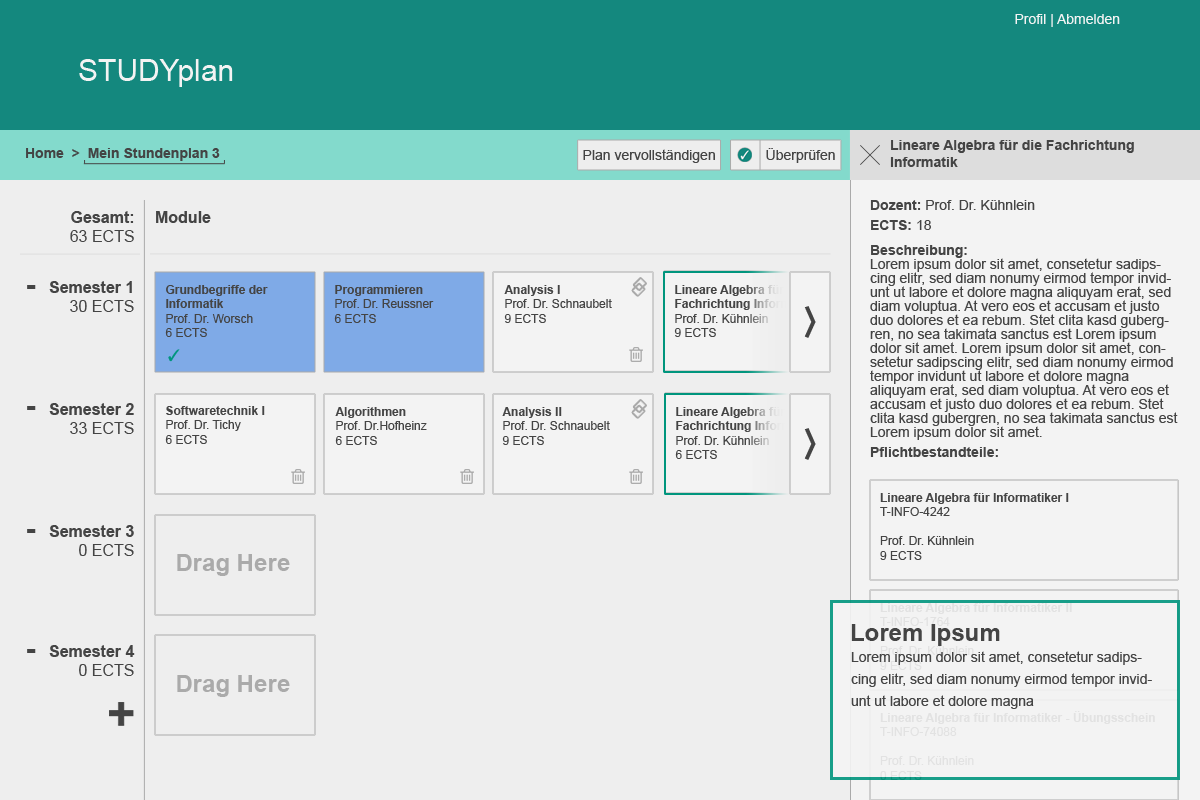
\includegraphics[width=0.7\textwidth]{../GUI/ergebnisse/verifizierung-1.png}
\end{figure}
\begin{figure}[!htb]
	\caption{}
	\label{fig:gui-verifizierung-2}
	\centering
	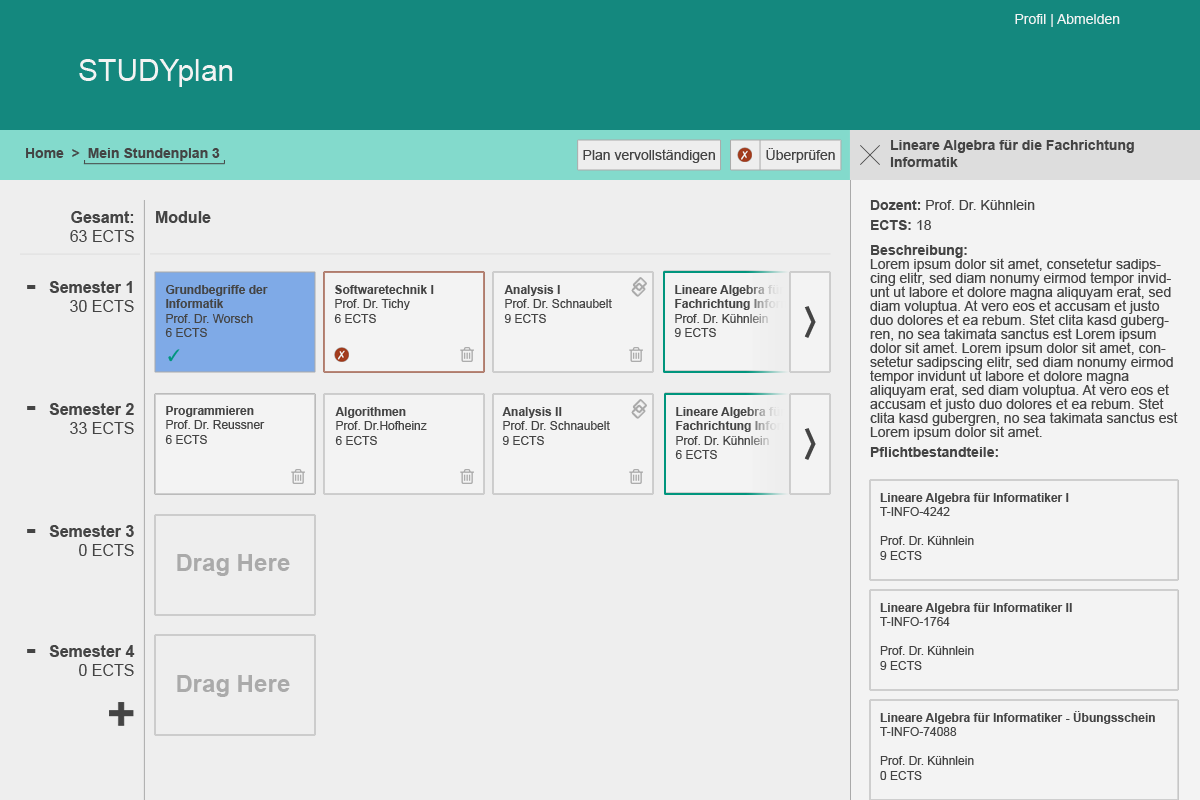
\includegraphics[width=0.7\textwidth]{../GUI/ergebnisse/verifizierung-2.png}
\end{figure}

\subsection{Profil}
So sieht das Profil aus.
\begin{figure}[!htb]
	\caption{}
	\label{fig:gui-profil-1}
	\centering
	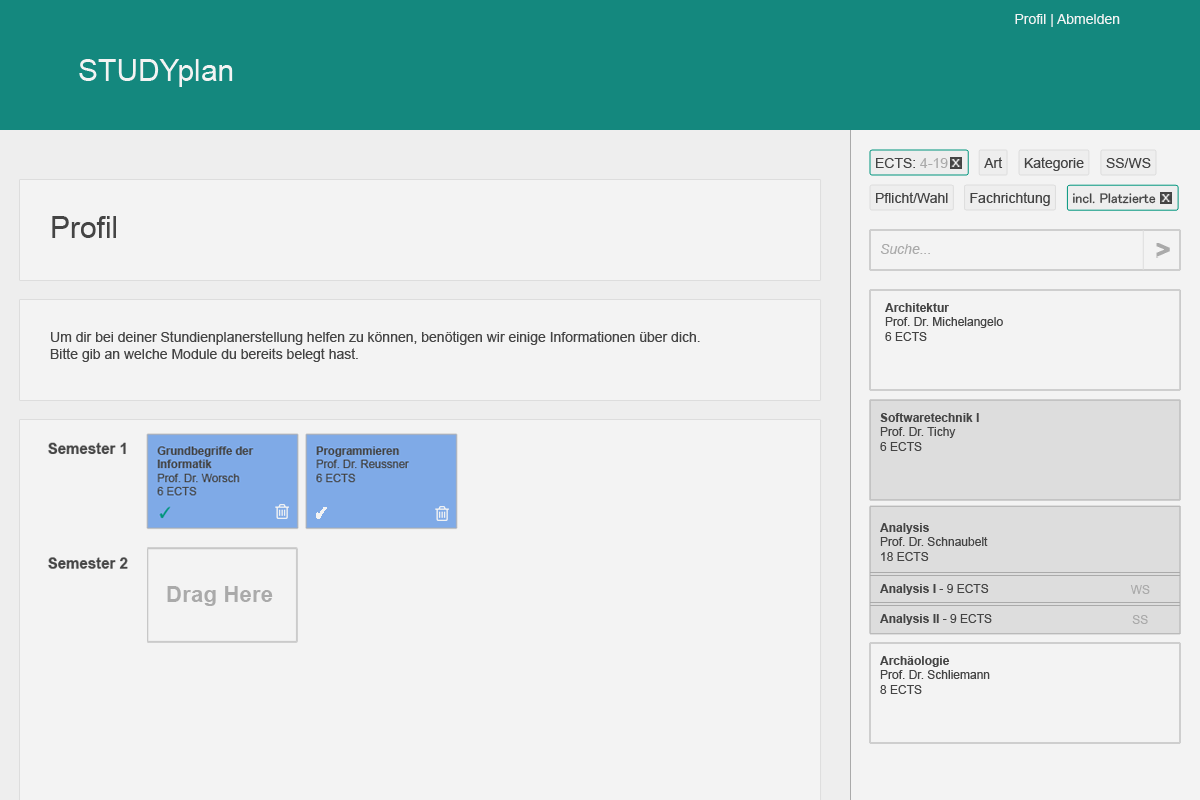
\includegraphics[width=0.7\textwidth]{../GUI/ergebnisse/profil-1.png}
\end{figure}